Determining the~expected number of~generated identifiers or the~number of~collisions in the~ECFP encoding for given parameters \( r \) and \( N \) requires making some assumptions about the~encoded molecular structure, at least about the~number of~vertices and edges in the~corresponding graph. Presumably, it would be possible to~estimate these values if knowing an algorithm for sampling random compounds. One method that might be used for this uses context-sensitive grammar to~define the~valid bonds between specific atoms and substructures \cite{sun2024grammars}. Then, the~result of~a~random walk on the~production graph determines the~correct structure. To ensure the~validity of~the conclusions, it would be needed to~prove that, for a~specific CSG, the~described method generates compounds from a~near-real distribution in terms of~their size and the~frequency of~occurrence of~specific substructures. It may thus be sufficient to~experimentally determine the~mean value of~the investigated parameters using a~large set of~real-world compounds.

The dataset consisted of~two subsets. The first subset consisted of~\( 2.4 \) million compounds from the~\href{https://www.ebi.ac.uk/chembl/explore/compounds/}{ChEMBL} database classified as bioactive. It contained structures of~different sizes with the~largest made out of~\( 681 \) atoms and an average of~\( 31 \) atoms. The second subset, containing only hydrocarbons, was generated using the~Wright, Richmond, Odlyzko, and McKay algorithm for enumeration of~all non-isomorphic unrooted trees for a~fixed number of~nodes. The exact implementation was the~one provided by \href{https://gist.github.com/hagberg/7979081}{Aric Hagberg}. The hydrocarbon dataset was chosen to~examine the~properties of~the ECFP encoding within the~family of~similar structures.

The ECFP encodings of~all the~compounds were computed using functions available in the \href{https://www.rdkit.org/docs/source/rdkit.Chem.rdMolDescriptors.html}{\texttt{rdkit.Chem.rdMolDescriptors}} module with parameters \( r \in \set{1, \ 2, \ 3} \), \( N \in \set{1024, \ 2048, \ 4096, \linebreak 8192} \) as the~most commonly used values \cite{chemaxon2025docs, le2020decipher}.
\begin{figure}[H]
    \centering
    \begin{subfigure}[!t]{0.5\textwidth}
        \centering
        a) The random dataset
        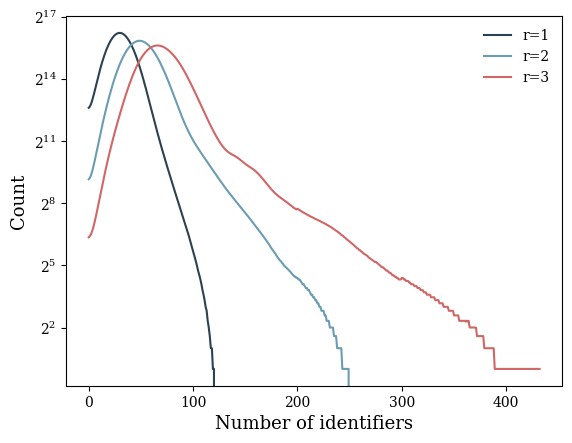
\includegraphics[height=5.4cm]{figures/num_bits}
    \end{subfigure}%
    ~
    \begin{subfigure}[!t]{0.5\textwidth}
        \centering
        b) The hydrocarbon dataset
        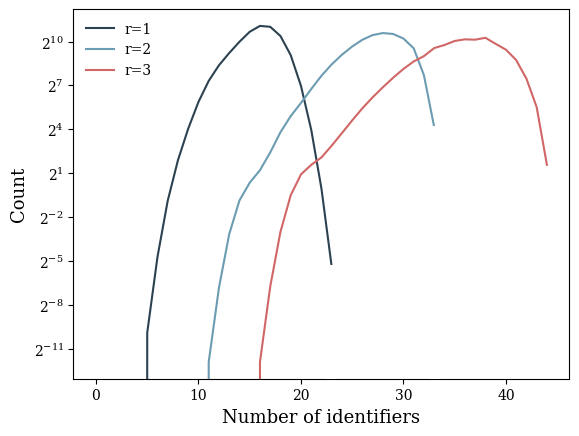
\includegraphics[height=5.4cm]{figures/num_bits_c22}
    \end{subfigure}
    \caption{Number of identifiers generated in the ECFP procedure}
    \label{fig:num_bits}
\end{figure}

The longest encoding for \( r=3 \), in the random dataset, contained \( 432 \) identifiers. As expected, the~encodings of the set of hydrocarbons had a distribution more concentrated around the~mean, as~the range of the number of identifiers was between \( 9 \) and \( 45 \). Comparing the results to~the length of the encoding \( N \approx 10^3 \), the~representation is sparse -- even more so in the average case and for smaller \( r \). Despite this, when projecting identifiers onto a~binary vector of a fixed length some collisions may occur.
\begin{figure}[H]
    \centering
    a) The random dataset
    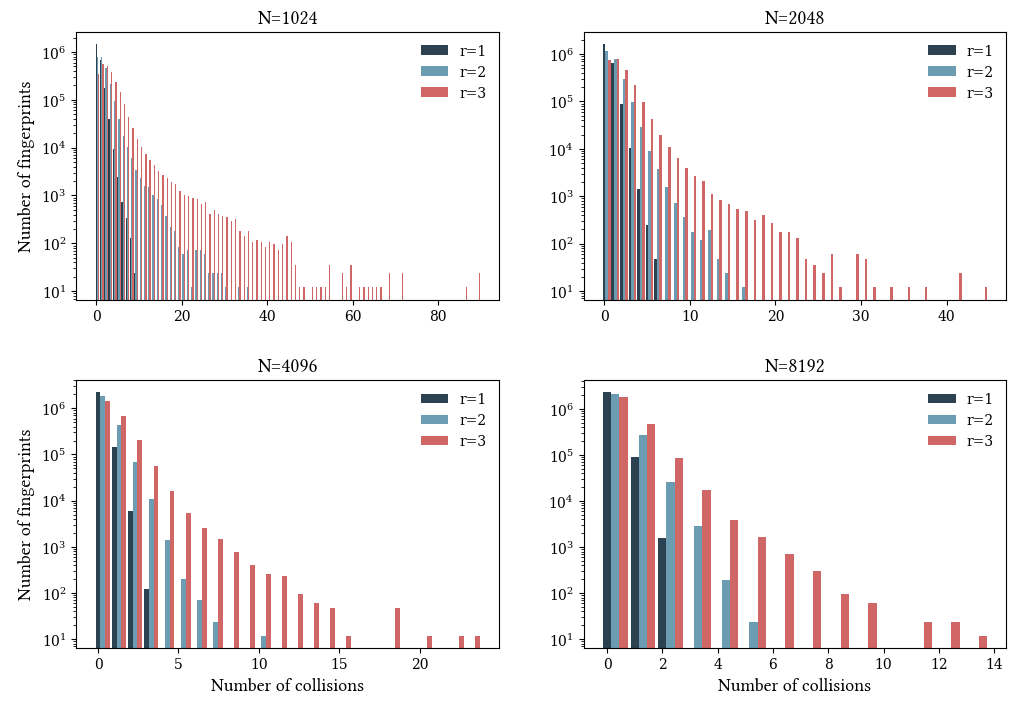
\includegraphics[width=0.95\textwidth]{figures/num_collisions.png}
\end{figure}
\begin{figure}[H]
    \centering
    b) The hydrocarbon set
    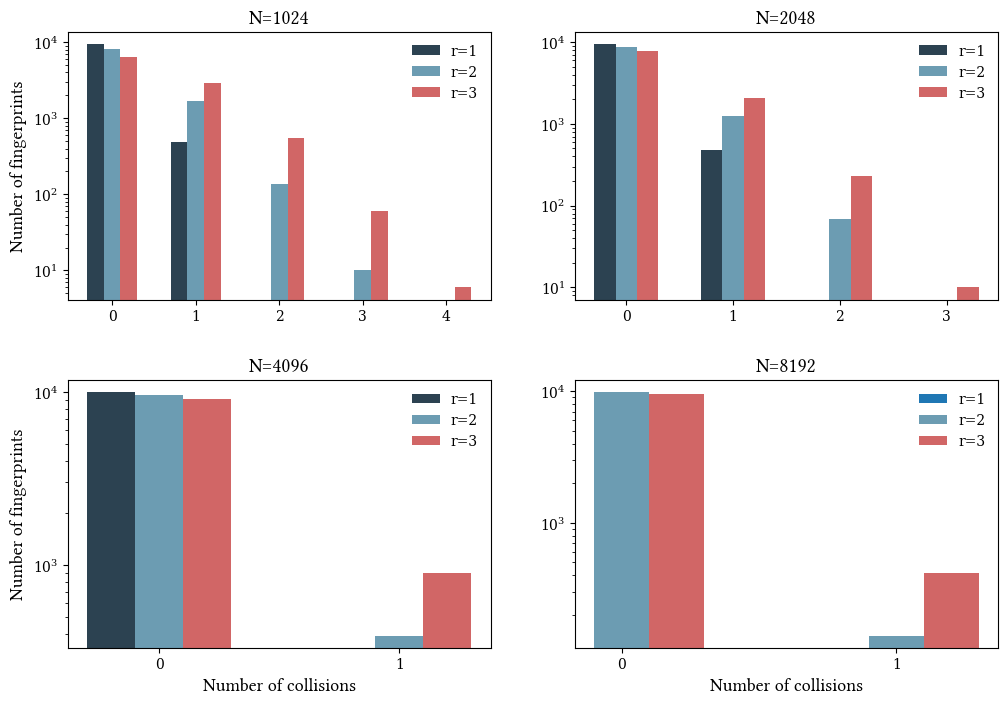
\includegraphics[width=0.95\textwidth]{figures/num_collisions_c22.png}
    \caption{Number of~collisions due to~projection of~identifiers on a~vector depending on the~parameters \( r,\; N \) for a) random set b) hydrocarbon family}
    \label{fig:num_collisions}
\end{figure}
The average number of~collisions for all parameter configurations was less than 3, and for \( r=1 \) or for \( N \geq 4096 \) it was less than 1. This raises the~question of~how much collisions affect the~similarity coefficient.